%!TEX root = ../thesis.tex
\chapter{工程案例——上海地铁盾构隧道}
\label{chap:case}

本章以上海城市轨道交通12号线的天潼路至国际客运中心站区间为工程案例,以基础设施智慧服务系统(iS3)(朱合华等,\citeyear{朱合华2018智慧基础设施})为基础,介绍本文提出的盾构隧道服役性能评估与预测方法,及其微服务在iS3系统中的集成和应用。本文主要贡献是以微服务形式实现了iS3平台的服务层iS3-Core,同时实现了iS3-Desktop和iS3-Web两个应用层程序。

%%%%%%%%%%%%%%%%%%%%%%%%%%%%%%%%%%%%%%%%%%%%%%%%%%%%%%%%%%%%%%%%%%%
\section{工程概述}

该区间于2013年12月正式开通运营,为盾构法单圆隧道。隧道区间里程范围为SK22+473.443-SK23+924.353(单线长1450.910$m$)。该区间隧道内径为5500$mm$,外径为6200$mm$,共有1208环(含联络通道特殊管片)。衬砌采用预制钢筋混凝土管片,通过标准环+转弯环的组合方式通缝拼装。衬砌全环由小封顶F、两块标准块B、两块邻接块L及一块大封底块D共6块管片构成,分块角度为2B(65°)+2L(65°)+F(16°)+D(84°),环宽1200$mm$。管片强度等级C55、抗渗等级为S10。管片纵向和环向均采用直螺栓连接,管片环之间用17根M30的纵向螺栓相连接。工程平面图如图~\ref{fig:天潼路至国际客运中心站区间平面图}~所示。

\begin{figure}[htb!]
    \centering
    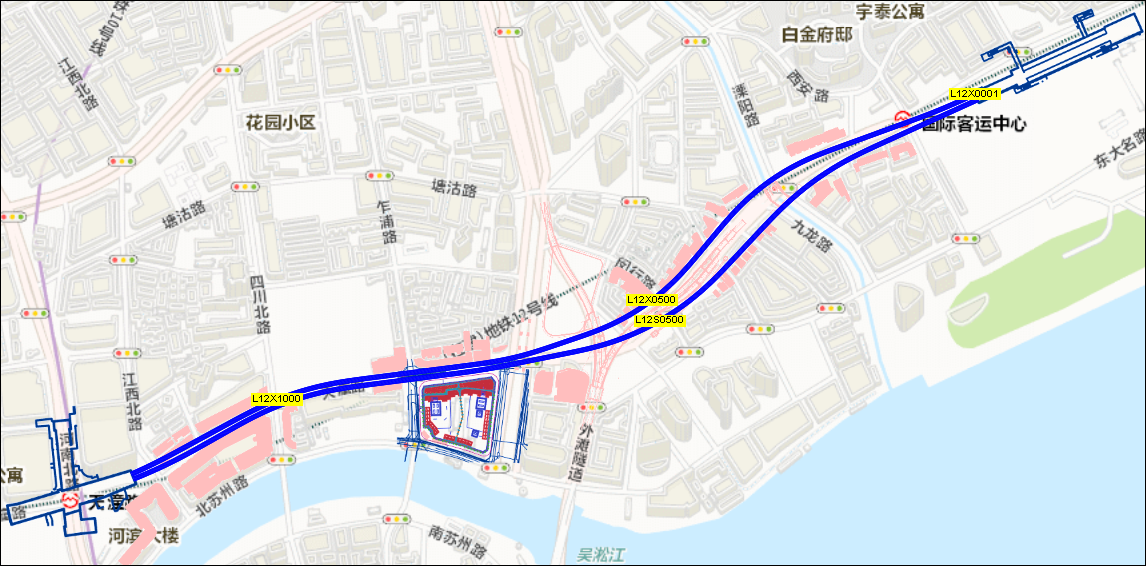
\includegraphics[width=0.9\textwidth]{chap5/plan-map.png}
    \caption{天潼路至国际客运中心站区间平面图}
    \label{fig:天潼路至国际客运中心站区间平面图}
\end{figure}

2016年3月末,在该上行区间沿线附近有“中美信托大厦”基坑开挖施工。基坑对应区间里程约SK22+950.2$m$-SK23+58.2$m$,对应上行线环号约720-810环,距离隧道水平距离最近处约10.3$m$。基坑总面积约1000$m^2$,普通区域下设四层地下室,邻近轨道交通区域设置两层地下室。采用顺作法施工,首先施工远离区间隧道的基坑,待该部分地下室施工完成后再开始施工邻近轨道交通侧基坑。

在基坑开挖期间,为降低基坑施工过程中对隧道结构可能产生的不利影响,保障城市地铁正常运营,对隧道结构变形进行监测,在隧道受影响区范围内布设无线双倾角传感器,用于监测管片的倾角变化,然后通过管片倾角变化量推算衬砌环的收敛变形。无线监测传感器在区间的布置里程为 SK22+716.2$m$-SK23+256.2$m$,对应管片环号555环-1005环,总长度为 540.0$m$。监测断面的布置基本思路是:在基坑正对的隧道区间内采取短间隔监测断面,并布设两种传感器,而在两端稍远范围内可以适当加大监测断面间距。以基坑影响核心区域为中心并向两侧延伸,共选取了19环监测断面。根据断面内的不同布设方案,监测断面分为三类,共计安装了50个双倾角传感器,如图~\ref{fig:天潼路至国际客运中心站区间平面图}~所示。

\begin{figure}[htbp] 
    \centering 
    \begin{tabular}{c} 
        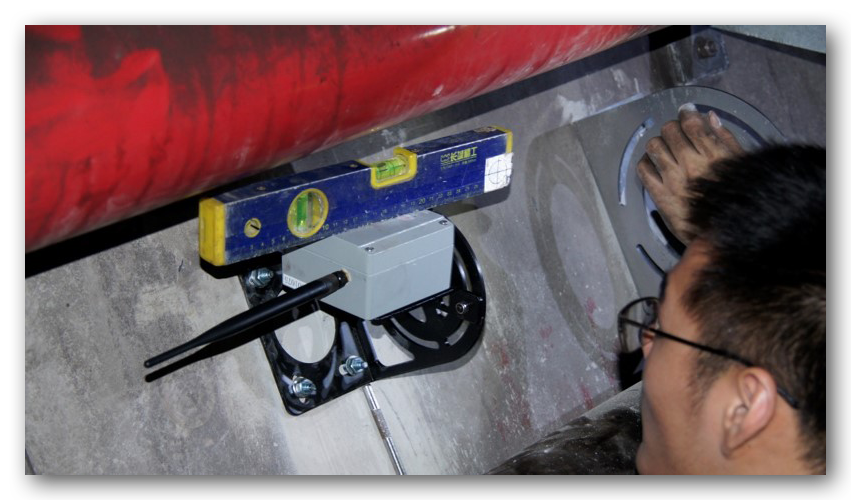
\includegraphics[width=0.8\textwidth]{chap5/sensor1.png} \\ 
        (a)~隧道现场安装的倾角传感器 \\
        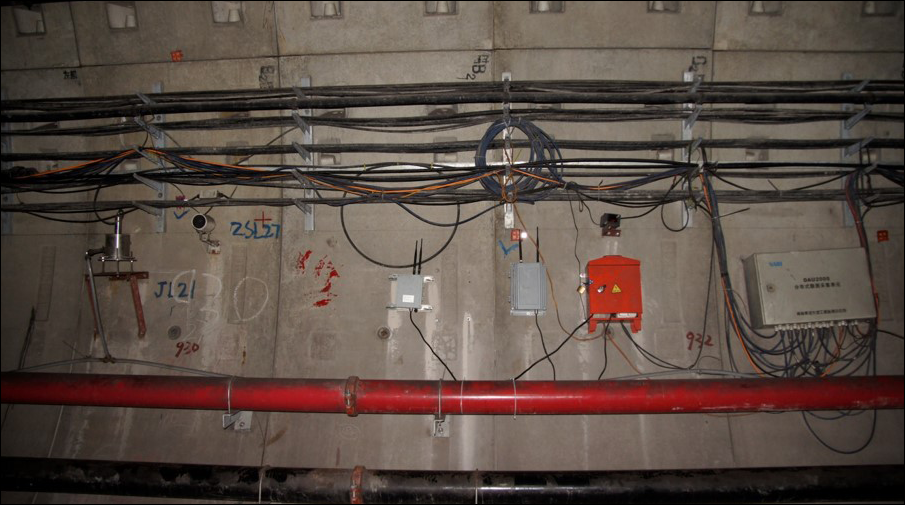
\includegraphics[width=0.8\textwidth]{chap5/sensor2.png} \\ 
        (b)~无线传感器系统的网关设备 \\
    \end{tabular}
    \caption{天潼路至国际客运中心站区间传感器安装示意图}
    \label{fig:天潼路至国际客运中心站区间传感器安装示意图} 
\end{figure}

%%%%%%%%%%%%%%%%%%%%%%%%%%%%%%%%%%%%%%%%%%%%%%%%%%%%%%%%%%%%%%%%%%%
\section{基础设施智慧服务系统(iS3)介绍}

\subsection{iS3系统基本概念}

iS3旨在从信息流角度对基础设施工程进行管理,是基础设施全寿命数据采集、处理、表达、分析的一体化决策服务系统。

数据采集是指利用各类传感器感知基础设施状态的过程,并将感知到的数据按一定规律变换成为电信号或其他所需的输出形式,以满足数据传输、处理、存储、显示、记录和控制等要求。数据采集方法是指利用各种途径、方式,获取工程建设、运营过程中所需的各种数据。

数据处理是对采集来的数据进行去伪存真、去粗取精、由表及里、由此及彼的加工过程,也是在原始基础设施数据的基础上,提取出价值含量高、方便用户利用的信息的活动过程。由于工程环境和认为因素等原因,采集的信息,掺杂了与基础设施结构工作性能及损伤状态无关的噪声,需要对数据进行处理。从基础设施监测数据中提取对象特征的方法主要有: 数字滤波技术、自适应卡尔曼滤波技术、小波分析技术、分形几何技术、模糊技术等。

数据表达包括建模(包括地质体、地下管线、建筑、结构、设备等建模)、仿真、可视化(例如虚拟现实和增强现实)、三维打印等。数据表达作为可视化手段,以视觉认知的方式地将工程数据呈现在用户面前; 利用数据分析手段进行数据查询及数据相关关系分析,发掘建设各阶段内和各阶段间的数据内在规律和特征; 利用动态采集及实时分析技术进行信息重构,以解决工程辅助设计、三维动态施工、工程监测与智能控制等工程建设问题。

数据分析是指在工程规划、勘察、设计、施工与运营全寿命数据基础上,通过物理数学方法实现工程问题的定性和定量分析。数据分析的目标和对象是多种多样的,相应的分析手段也是多种多样的,包括: 统计分析、空间分析、数字-数值一体化分析、人工智能分析、大数据分析、云计算与物计算、数据融合,以及多维度模拟分析、造价分析、建筑物理性能分析、施工动态反馈分析、工程风险分析、建养一体化分析、火灾动态预警分析和决策支持分析等等。

一体化决策服务系统表示针对基础设施的智慧化提供从数据采集、处理、表达、分析、服务与决策的集成解决方案。

\subsection{iS3系统整体框架}

iS3 可分为五个层次: 基础层、数据层、服务层、应用层和用户层,如图~\ref{fig:iS3系统框架图2}~所示。基础层是整个系统的硬件设备集合,包括运行iS3的服务器、执行云分析的高性能计算集群、数据采集所用的物联网传感器等设备,和联系这些设备的网络、基站,为其他层提供硬件层次的保障。

数据层是为服务层提供其所需的访问、计算和存储等资源。数据资源是多样化的,最基础的是数据库数据,由工程数据经“数字化”处理后存储在数据库中,工程的图形数据有二维模型和三维模型两种,主要以CAD、GIS和BIM等软件格式存储,除此之外数据层还包含原始文档数据。

服务层是为应用层提供数据访问接口、分析服务接口的逻辑层,由iS3服务(iS3 Core)提供,服务层一方面简化、统一了数据访问的方式和底层硬件设备的调用方式,另一方面则保证了数据的安全性,不被随意访问、改动和删除。

应用层即为面向用户的客户端程序,提供用户与系统的友好访问。iS3 中包含桌面端(iS3 Desktop)、Web端(iS3 Web)、移动端(iS3 Mobile)和云端(iS3 Cloud)等四种应用,满足用户使用的不同需求,可为用户提供实时数据查询、可视化浏览、数据分析、结构分析等功能。

用户层是使用基础设施智慧服务系统的群体,包括业主、设计、施工、运维、科研人员等。

本文主要贡献是以微服务形式实现了iS3平台的服务层iS3-Core,同时实现了iS3-Desktop和iS3-Web两个应用层程序。

\begin{figure}[htb!]
    \centering
    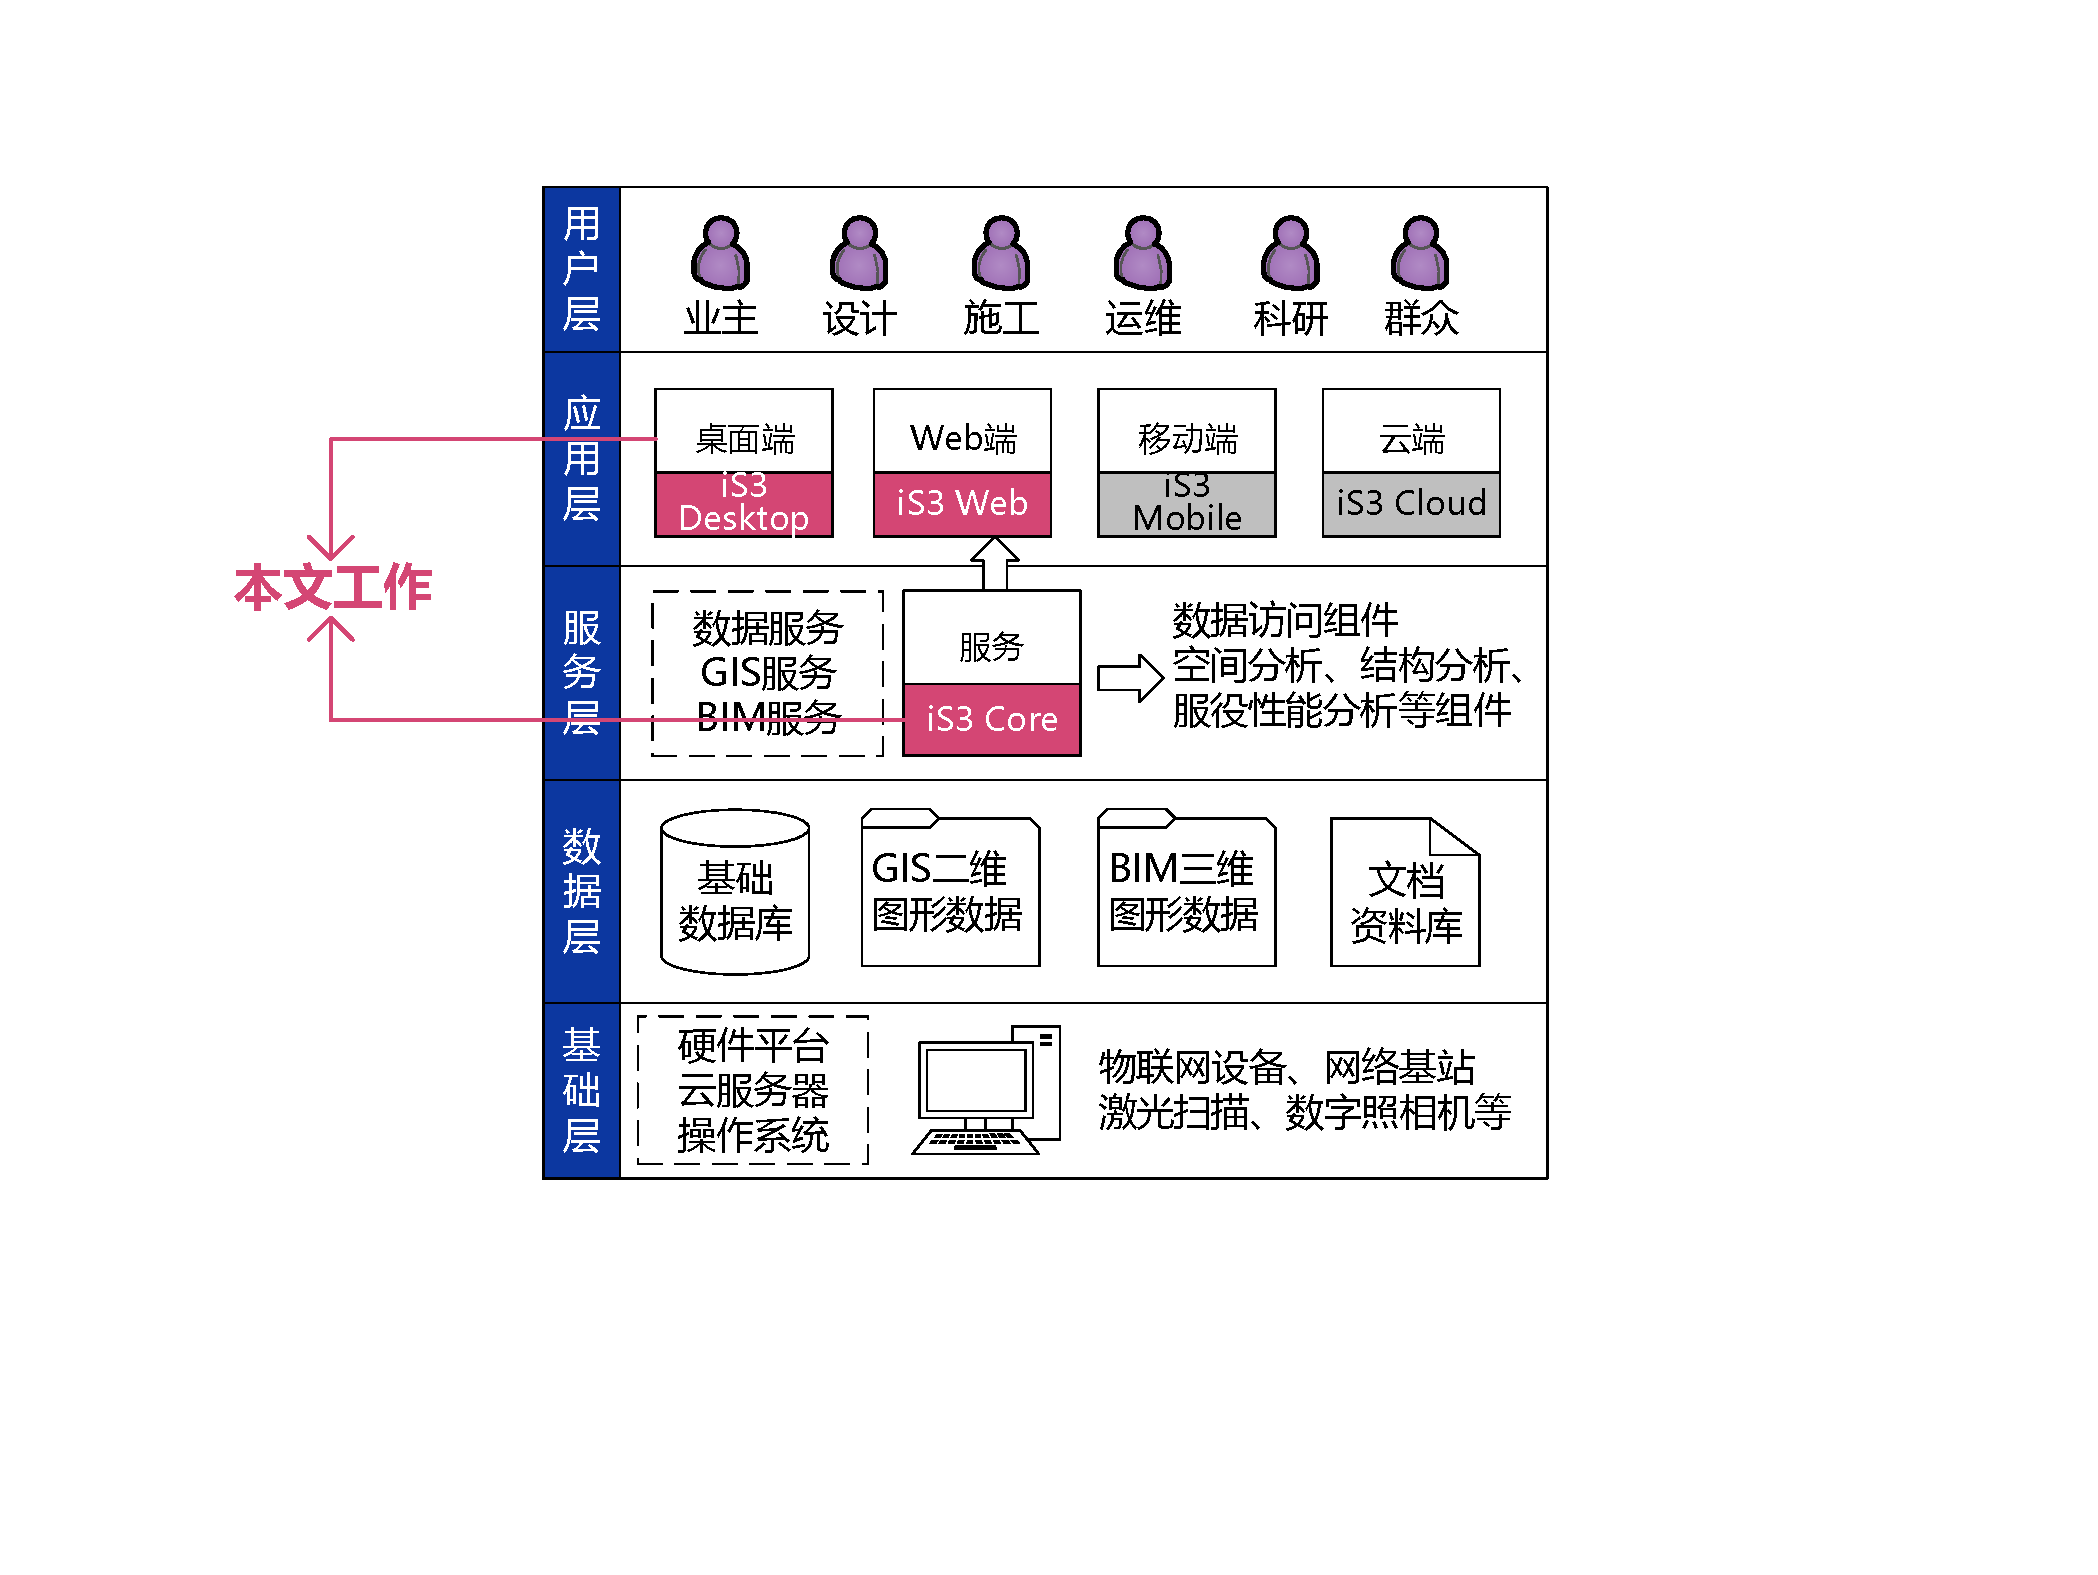
\includegraphics[width=0.9\textwidth]{chap5/iS3-framwork.pdf}
    \caption{iS3系统框架图}
    \label{fig:iS3系统框架图2}
\end{figure}

%%%%%%%%%%%%%%%%%%%%%%%%%%%%%%%%%%%%%%%%%%%%%%%%%%%%%%%%%%%%%%%%%%%
\section{服役性能评估与预测服务应用}

\subsection{服务发现中心}

服务发现中心的主要作用是管理所有的微服务,管理界面如图~\ref{fig:服务发现中心}~所示。作为示范工程,本文实现了五个微服务:API网关、数据微服务、有限元微服务、服役性能微服务和测试微服务,均部署在单机机器上。各个微服务启动后会向服务发现中心发送注册请求,服务发现中心的主界面能查询到正在运行的微服务,在实际应用中,调用某一微服务只需向服务发现中心请求该微服务的id,服务发现中心返回对应的微服务的ip地址和端口号。

根据第~\ref{chap:service}~章内容,数据微服务(Data-MS)主要提供监测检测数据的查询获取,有限元微服务(FEM-MS)实现了盾构隧道荷载结构模型和地层结构模型两种方法,服役性能微服务(TSI-MS)则实现了TSI指标的计算和沉降数据的时间序列模型。调用Eureka服务中心有两种方式,一种是借助Eureka客户端,其封装了根据微服务id获取分析服务的功能,目前Eureka客户端已支持多种开发语言,如Java语言的Eureka Client(Apache,\citeyear{eurekaclient2018}),JavaScript语言的Eureka JS Client(Jquatier,\citeyear{eurekajsclient2018}),Python语言的Eureka Python(KristianOellegaard,\citeyear{pythoneureka2018})和C\#语言的Steeltoe Discovery(Steeltoe,\citeyear{steeltoe2018});另外一种则是通过API网关,API网关其实是把Java版的Eureka Client封装成HTTP请求的更通用的调用方式。本文主要以第二种方式进行调用。

\begin{figure}[htb!]
    \centering
    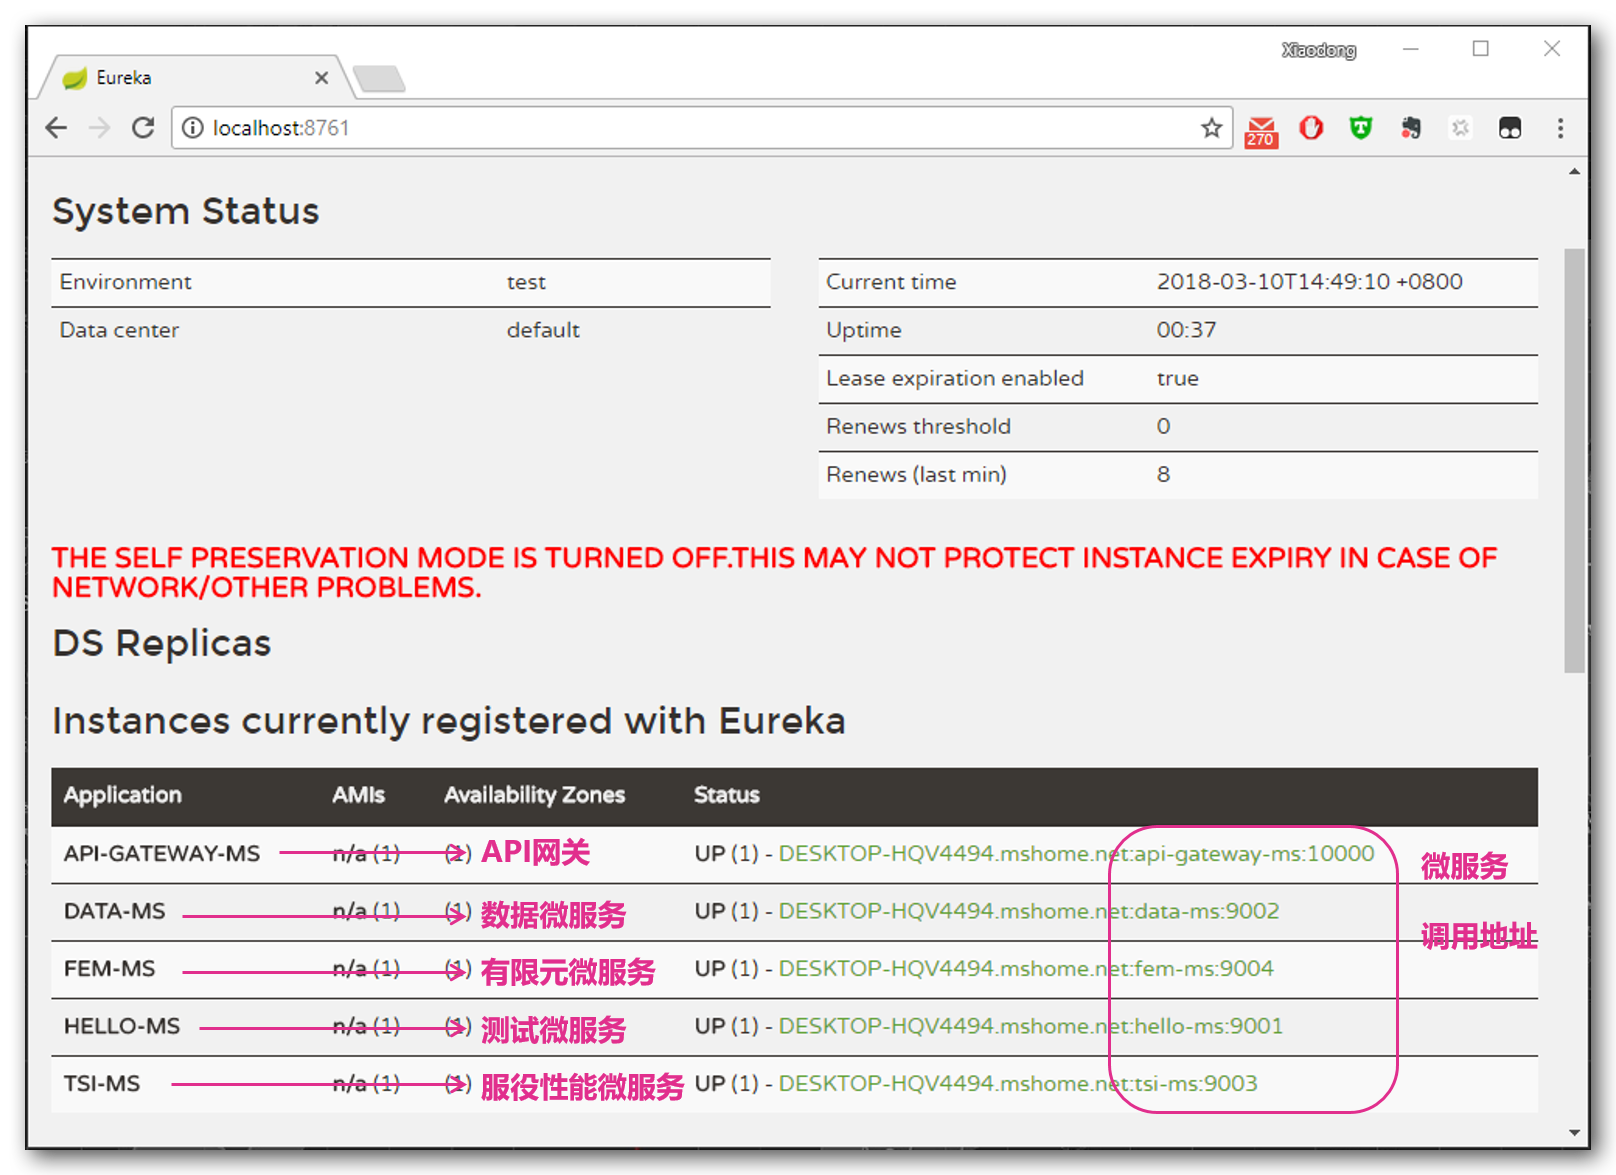
\includegraphics[width=0.85\textwidth]{chap5/discovery.png}
    \caption{服务发现中心}
    \label{fig:服务发现中心}
\end{figure}

\subsection{服役性能服务请求方式}
\label{chap:http-request-way}

大部分程序中都实现了HTTP请求功能,这一小节将介绍不同的HTTP请求方式,以获取示范工程的某一钻孔数据为例,其请求url为:http://localhost:9002/api/geology/borehole/1201。最简单的HTTP请求方式是通过浏览器,只需输入对应的url即可获取结果,如图~\ref{fig:浏览器的HTTP请求}~所示。从图中可获取id为1201的地质钻孔所有相关数据信息。

\begin{figure}[htb!]
    \centering
    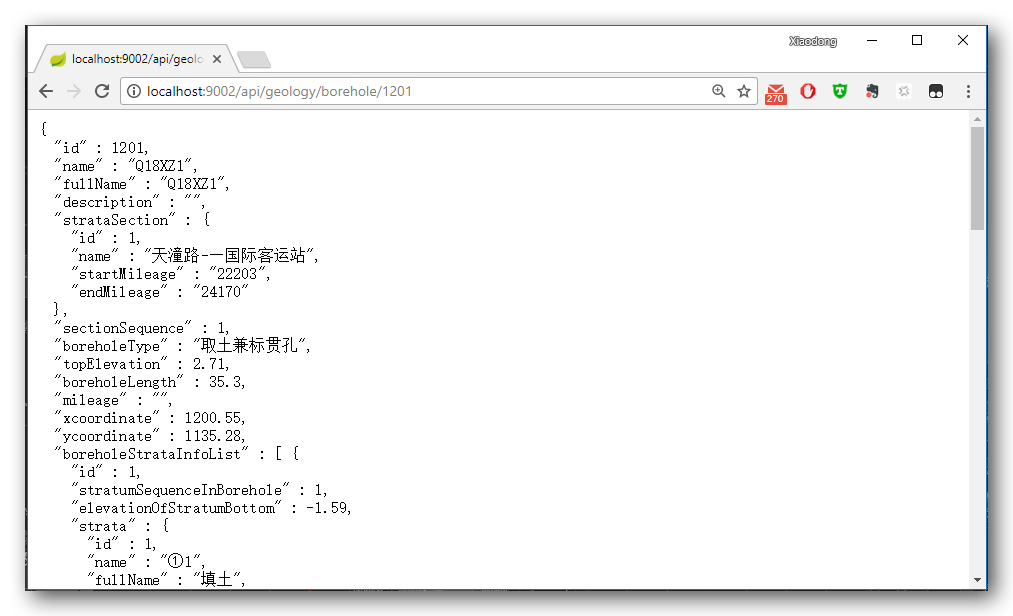
\includegraphics[width=0.85\textwidth]{chap5/browser-get.png}
    \caption{浏览器的HTTP请求}
    \label{fig:浏览器的HTTP请求}
\end{figure}

在操作系统中,可采用cURL命令进行HTTP请求,类Unix系统自带cURL命令,Windows系统则需自行安装该命令行,获取的结果与浏览器一样,如图~\ref{fig:命令行的HTTP请求}~所示。

\begin{figure}[htb!]
    \centering
    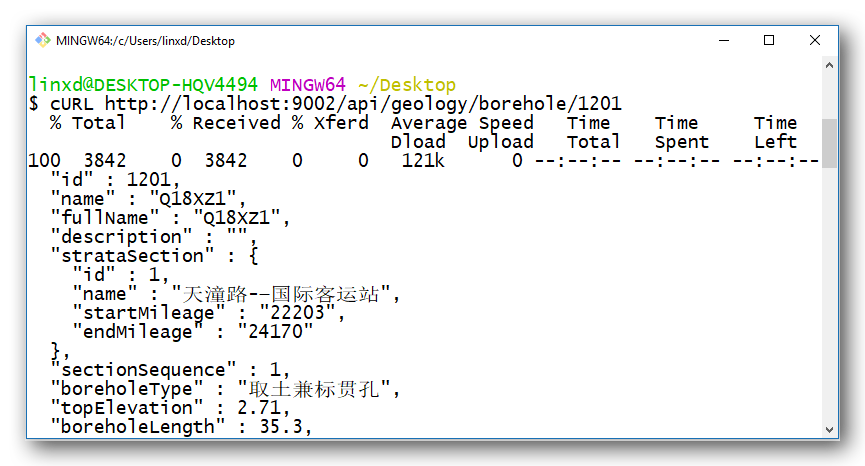
\includegraphics[width=0.85\textwidth]{chap5/curl-get.png}
    \caption{命令行的HTTP请求}
    \label{fig:命令行的HTTP请求}
\end{figure}

也可以借助第三方软件,如Postman(Google,\citeyear{postman2018})是google开发的一款功能强大的网页调试与发送网页HTTP请求,可以模拟各种HTTP请求,从常用的GET、POST到RESTful的PUT、DELETE等,请求结果如图~\ref{fig:Postman的HTTP请求}~所示。

\begin{figure}[htb!]
    \centering
    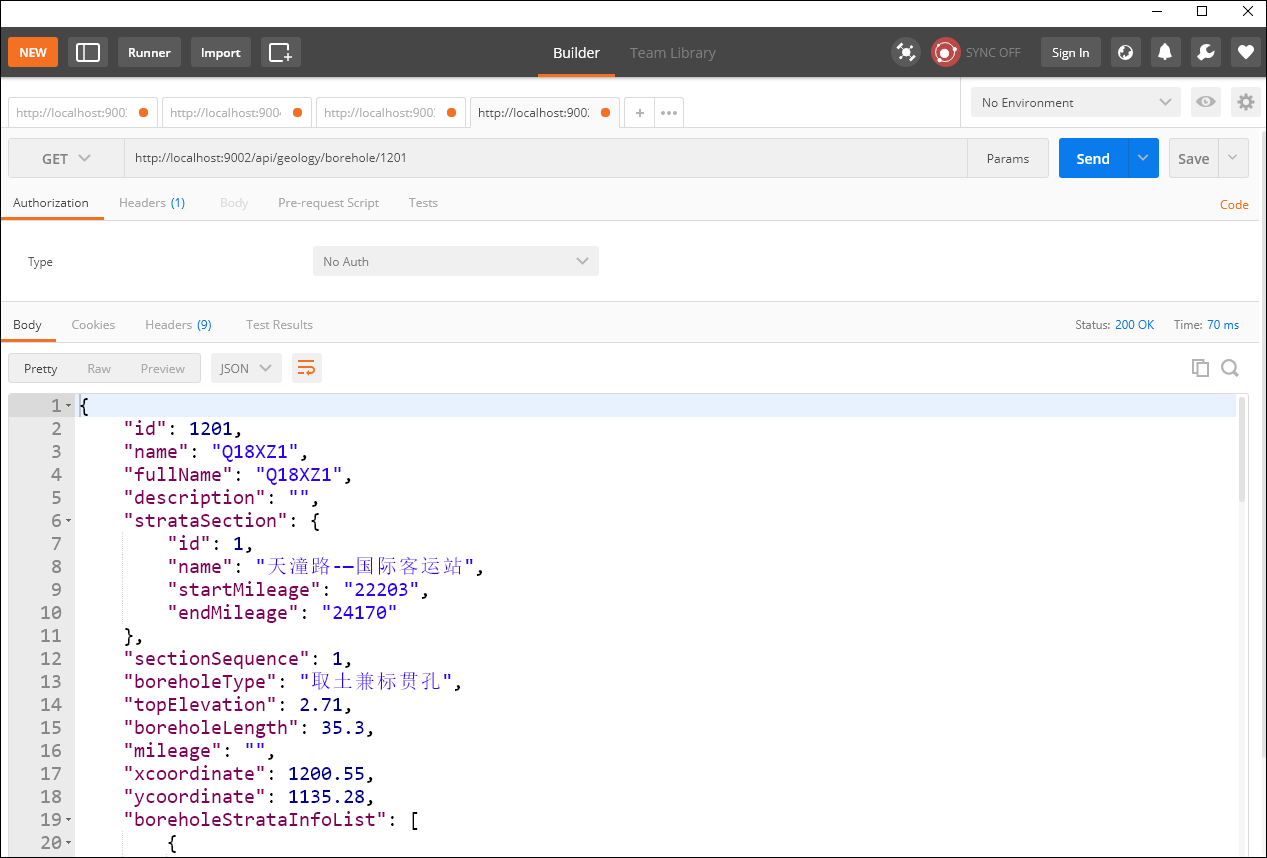
\includegraphics[width=0.85\textwidth]{chap5/postman-get.png}
    \caption{Postman的HTTP请求}
    \label{fig:Postman的HTTP请求}
\end{figure}

\subsection{服役性能相关微服务实现}

本节以Postman为例,说明实现的隧道服役性能相关的微服务接口形式,在第~\ref{chap:http-request-way}~小节已经示例了数据查询获取,隧道服役性能计算的请求结果如图~\ref{fig:隧道服役性能分析请求}~所示,图中请求参数有相对沉降、差异沉降、收敛变形、渗漏水、裂缝和剥落,dynamic参数决定计算方式是否引入动态变权。

\begin{figure}[htb!]
    \centering
    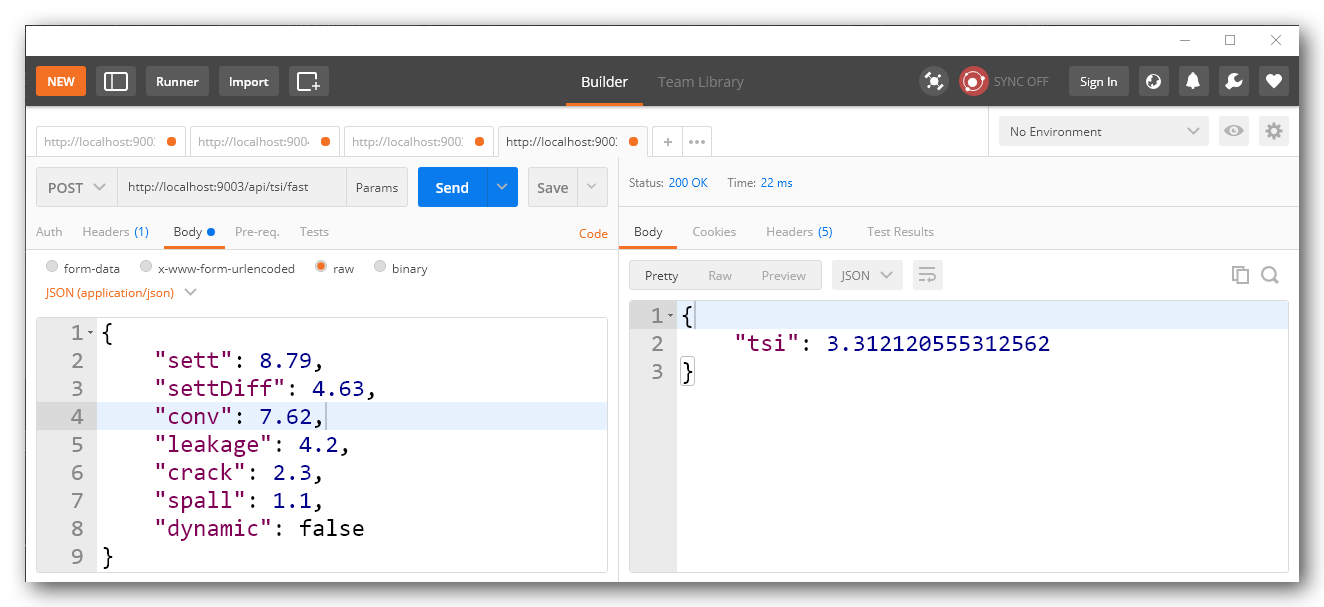
\includegraphics[width=0.85\textwidth]{chap5/tsi-post.png}
    \caption{隧道服役性能分析请求}
    \label{fig:隧道服役性能分析请求}
\end{figure}

图~\ref{fig:沉降时间序列模型分析请求}~为盾构隧道沉降数据的时间序列模型分析请求的结果,请求发送的数据包含历史沉降数据数组,和沉降数据的预测次数,响应数据为预测的沉降序列,由于迭代计算的原因,响应数据的前五组数据为0。

\begin{figure}[htb!]
    \centering
    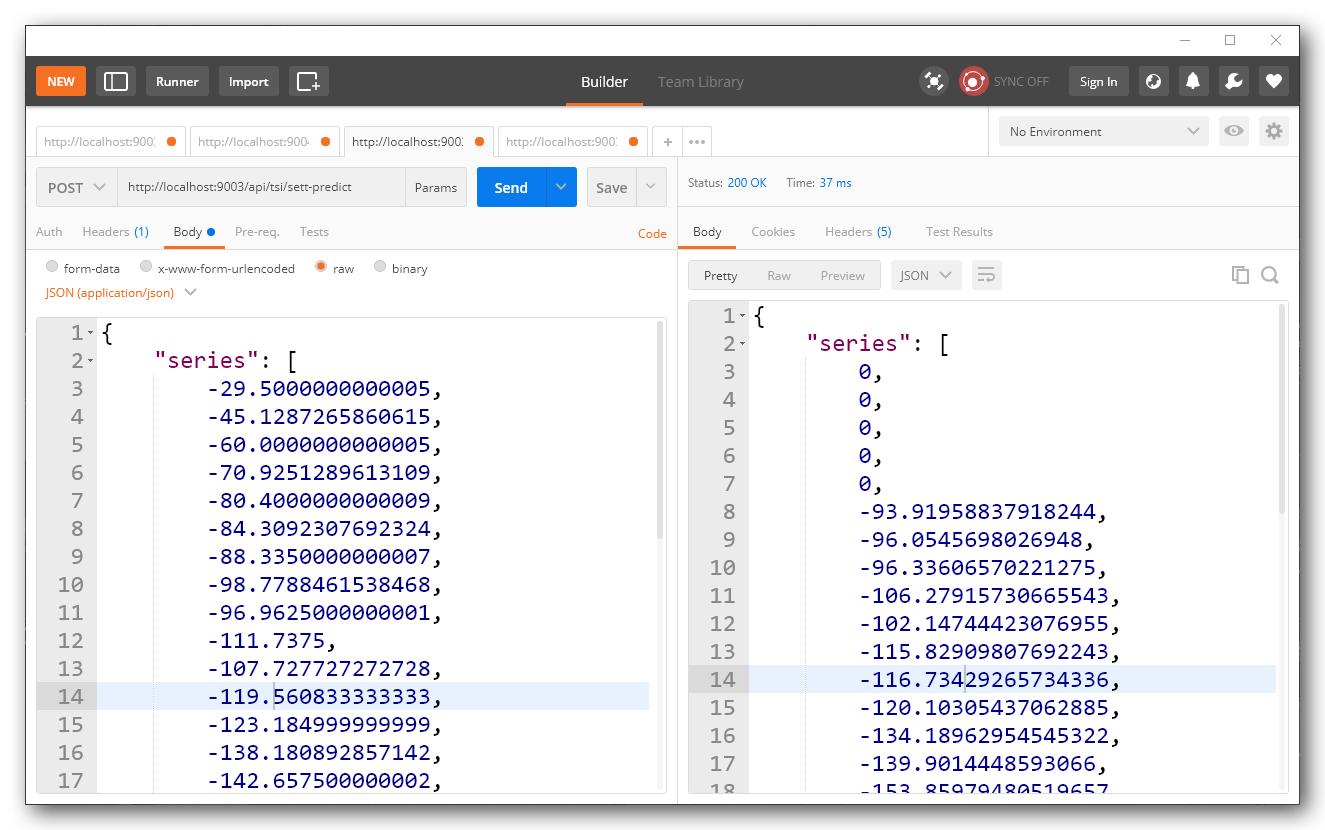
\includegraphics[width=0.85\textwidth]{chap5/time-series-post.png}
    \caption{沉降时间序列模型分析请求}
    \label{fig:沉降时间序列模型分析请求}
\end{figure}

有限元分析的微服务调用也类似,请求数据包含盾构隧道的基本信息,如隧道尺寸、材料属性、荷载信息等,服务端接收到请求后,在后台构件盾构隧道荷载结构法有限元模型,并提交Ansys进行分析,待解析结束后读取结果文件数据,并作为响应数据返回,包括模型节点的坐标与其内力数据。如图~\ref{fig:荷载结构有限元模型分析请求}~。

\begin{figure}[htb!]
    \centering
    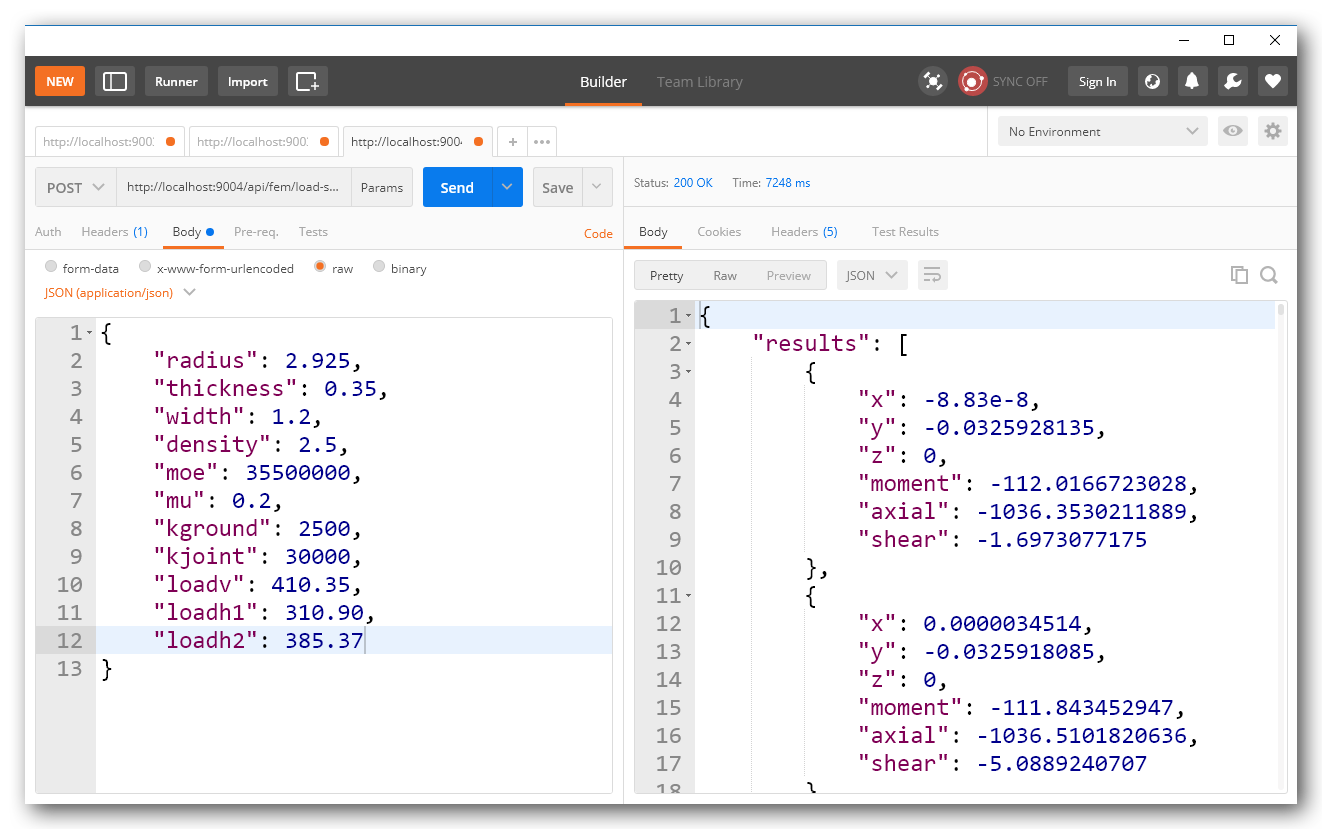
\includegraphics[width=0.85\textwidth]{chap5/fem-post.png}
    \caption{荷载结构有限元模型分析请求}
    \label{fig:荷载结构有限元模型分析请求}
\end{figure}

%%%%%%%%%%%%%%%%%%%%%%%%%%%%%%%%%%%%%%%%%%%%%%%%%%%%%%%%%%%%%%%%%%%
\section{微服务与iS3平台的集成}

基础设施智慧服务系统的应用层是直接与客户进行交互的,具备形象的用户界面和方面的操作方式,上述的微服务则是作为服务层为不同应用提供公共服务。规划的应用层包含了桌面端、网页端、移动端和云端几类,笔者限于时间原因,仅实现桌面端和网页端的部分功能。

\subsection{iS3桌面端}

桌面端iS3 Desktop界面如图~\ref{fig:iS3Desktop软件界面}~所示,展示了工程平面图(GIS几何模型,左窗口)、三维视图(BIM几何模型,右窗口)和统一信息模型数据(属性数据,下窗口)。图中示意了几何模型与数据根据统一编码关联的结果,在GIS和BIM的几何建模过程中,对构件赋予了唯一编码,可与统一数据模型关联。例如当在系统选中编码为GEO-BHL-1243的钻孔,所有窗口都能同时高亮显示该钻孔。同时也示意了在iS3 Desktop中请求服役性能微服务的窗口,发送请求数据获取TSI结果。

\begin{figure}[htb!]
    \centering
    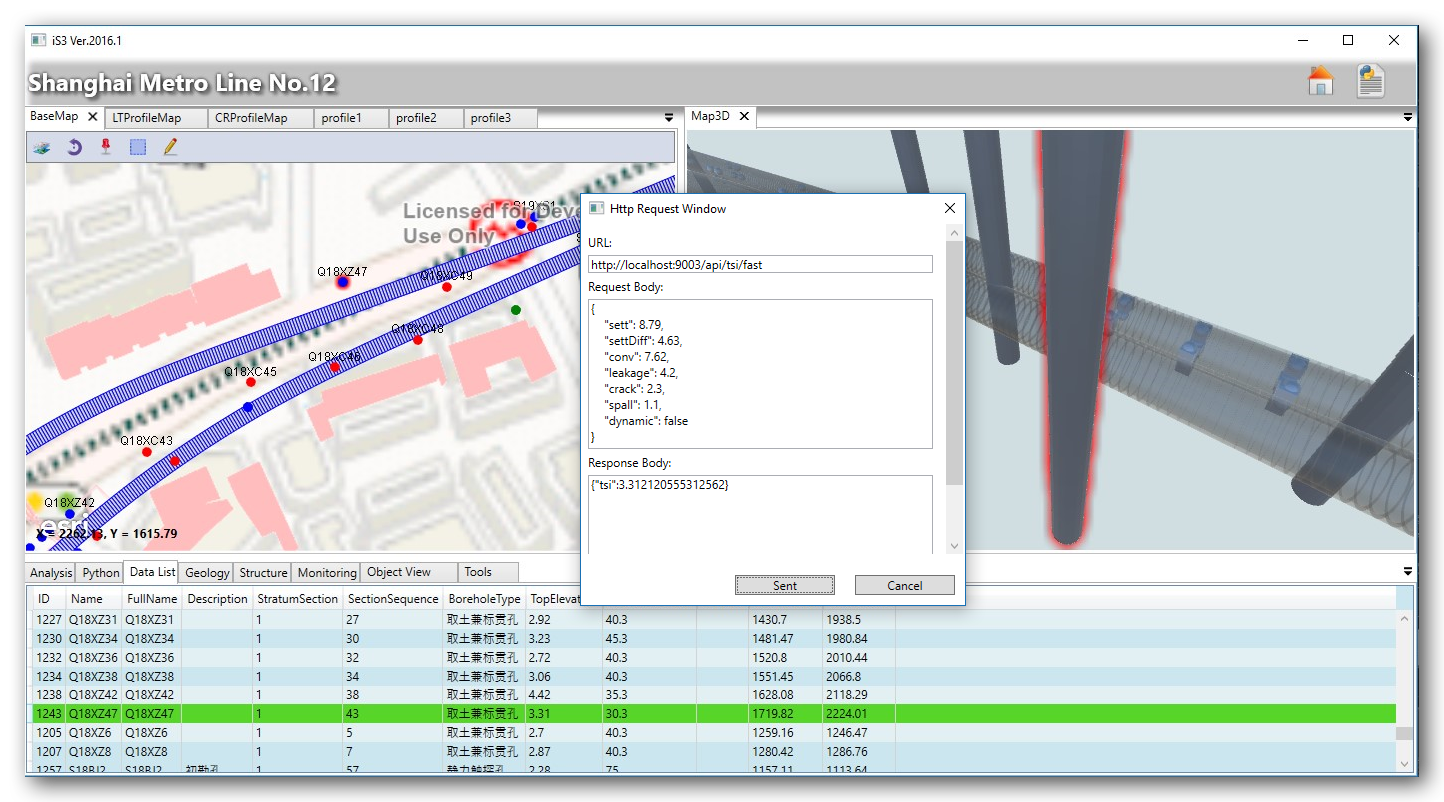
\includegraphics[width=0.9\textwidth]{chap5/desktop-planmap.png}
    \caption{iS3 Desktop软件界面}
    \label{fig:iS3Desktop软件界面}
\end{figure}

iS3 Desktop的信息模型可由数据微服务获取,对于地质勘察信息可获取钻孔深度、地层分布、土性描述、地层的各项物理力学特性统计指标等,从几何模型中可得到钻孔的坐标、空间相对位置等信息,如在系统中可高效获取编码为GEO-BHL-1218,名字为Q18XC22的钻孔的土层信息,即2.26至0.86$m$为灰黄色粉质粘土,0.86至-9.04$m$为灰色粘质粉土,-9.04至-13.49$m$为灰色淤泥质粘土,-13.49至-19.94$m$为灰色粘土,-19.94至-24.44$m$为灰色粉质粘土,-24.44至-40.54$m$为灰色砂质粉土夹粉质粘土,图~\ref{fig:地质勘察数据的可视化}~展示了开挖基坑周围的地层钻孔空间位置(中间窗口)、钻孔数据的统一数据模型(下边窗口)和根据地质信息绘制的选中的钻孔图(右边窗口)。用户可选择感兴趣隧道区段周围的钻孔,并定义地层的剖切面,系统将选中钻孔垂直投影至剖切面上,并根据相邻钻孔的土层信息对钻孔之间地层进行插值计算,最终由每个钻孔土层分布数据和钻孔空间位置可分析得到地质剖面图(左边窗口)。在隧道勘察阶段可利用系统对隧道周围地质情况进行充分的了解。

\begin{figure}[htb!]
    \centering
    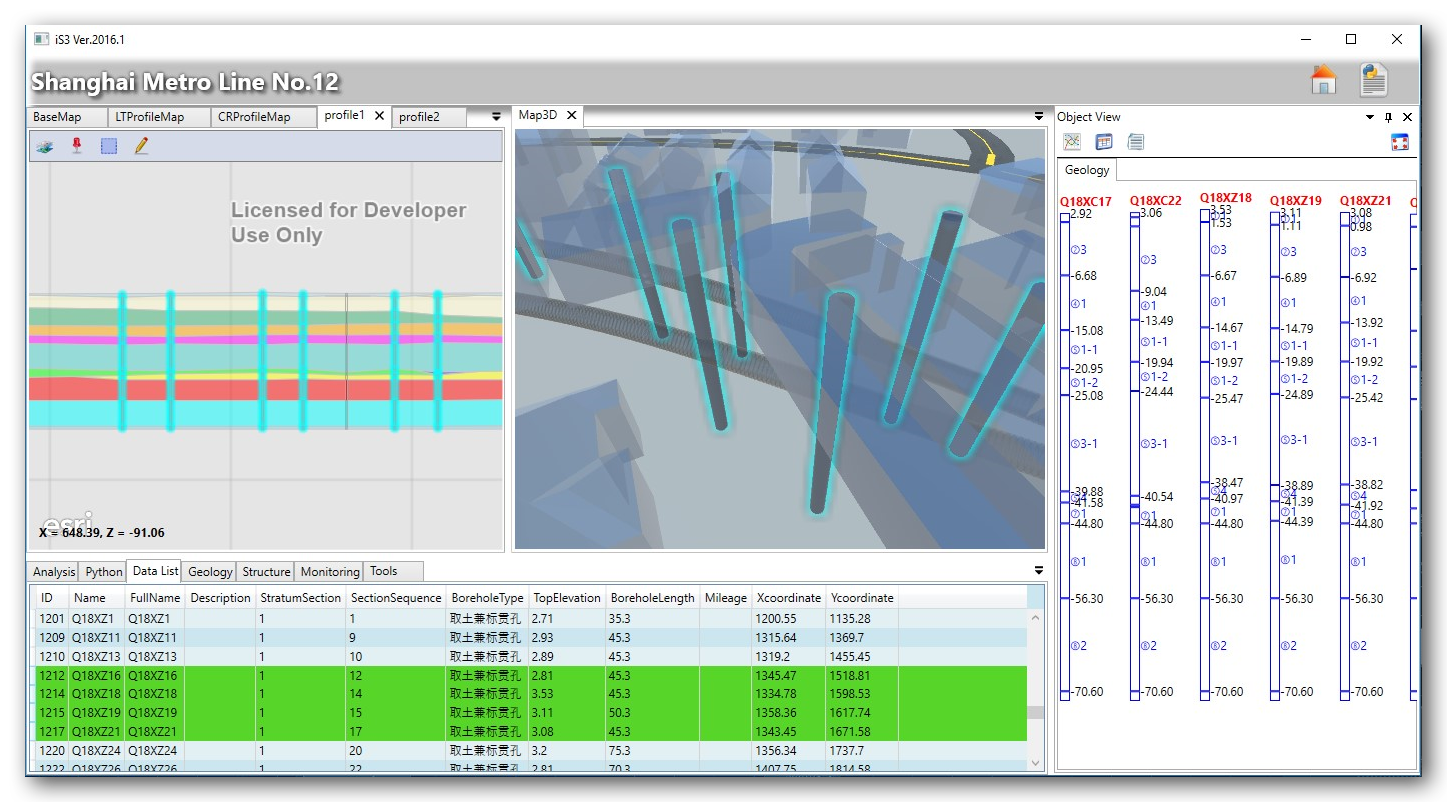
\includegraphics[width=0.9\textwidth]{chap5/desktop-geology.png}
    \caption{地质勘察数据的可视化}
    \label{fig:地质勘察数据的可视化}
\end{figure}

\begin{figure}[htb!]
    \centering
    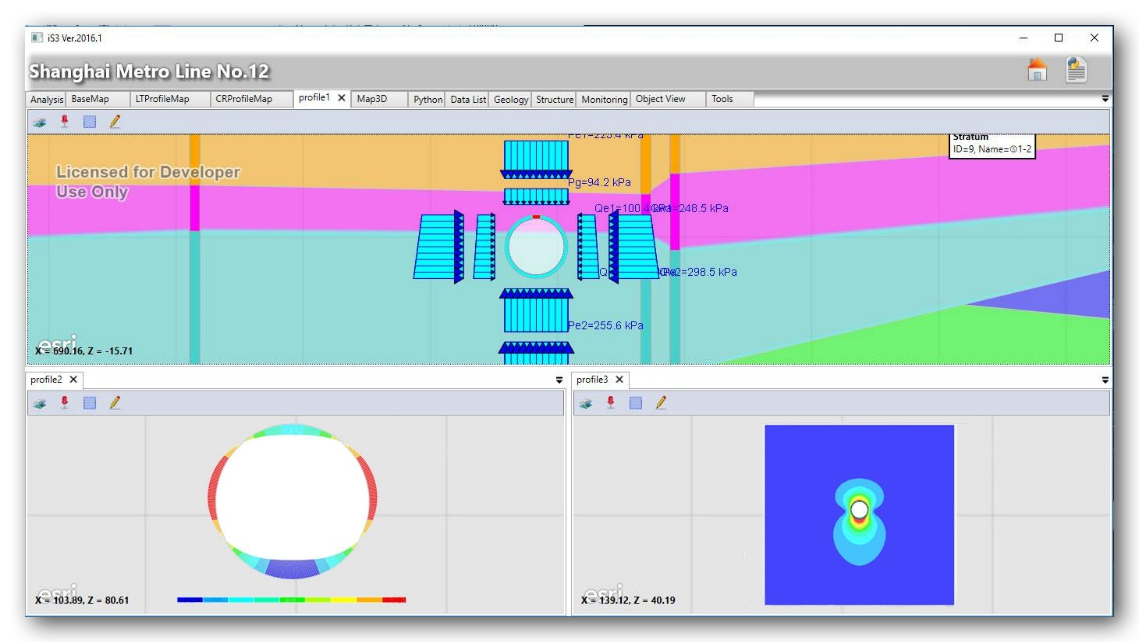
\includegraphics[width=0.9\textwidth]{chap5/desktop-structure.png}
    \caption{盾构隧道结构分析示意图}
    \label{fig:盾构隧道结构分析示意图}
\end{figure}

结构信息包括了隧道线路的平曲线组成、竖曲线组成、轴线里程、衬砌分块情况、管片材料、物理力学参数等,由几何模型和空间分析功能,可提取空间上有用信息数据,如范围查询、长度面积测量、缓冲区分析等,如图~\ref{fig:盾构隧道结构分析示意图}~。在隧道地质剖面分析基础上,将某一环衬砌垂直投影至剖面图,并利用空间分析功能可计算衬砌上覆各层土层厚度,由上覆土层物理力学参数,分析隧道周围水土荷载的结果(上边窗口)。另外系统也实现了有限元分析的功能,以荷载结构法为例,盾构隧道管理系统将衬砌尺寸、材料属性和分析得到的垂直荷载和水平压力,以HTTP请求方式发送至有限元分析微服务,返回的分析结果包括数值模型节点坐标、弯矩、轴力和剪力等信息,结果数据可视化效果(左下窗口),类似的,可实现地层结构法(右下窗口)的分析,为隧道结构设计提供参考。

监测信息则包含了隧道沉降、收敛、倾角等监测信息。工程案例采用无线传感器进行实时采集,在服务器上部署专门的接收程序接收网关的数据,再将原始数据通过数据微服务保存至本系统的信息模型。无线采集通过在开挖基坑影响范围内的隧道布设双倾角传感器,用于监测管片的倾角变化,通过管片倾角变化量计算衬砌环的纵向变形和环向变形,如图~\ref{fig:盾构隧道运营监测信息}~所示,无线传感器二维布置事宜图(左上窗口)和三维布置示意图(右上窗口),通过在几何模型中选取对应的监测点,可在显示近期的监测数据图表(右下窗口)。

\begin{figure}[htb!]
    \centering
    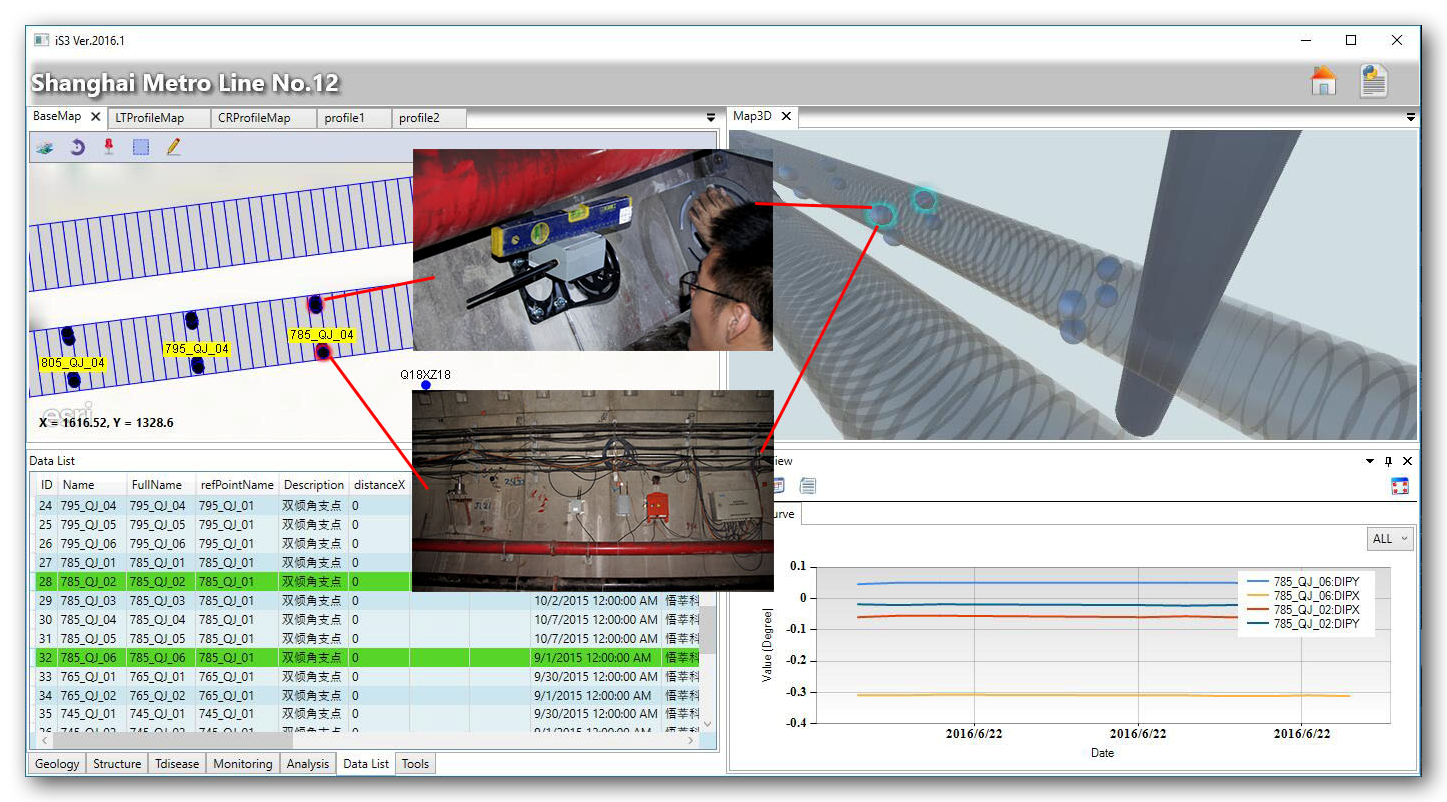
\includegraphics[width=0.9\textwidth]{chap5/desktop-monitoring.png}
    \caption{盾构隧道运营监测信息}
    \label{fig:盾构隧道运营监测信息}
\end{figure}

在维护养护阶段,根据信息模型中的监测检测信息,获取该区间的沉降大小在0-9 mm,收敛变形大小在0-10‰D(D为衬砌直径),区间总共有19处渗漏水、23处裂缝和12处剥落,调用服役性能微服务分析接口可计算得到区间隧道的服役性能数值大小,如图~\ref{fig:盾构隧道服役性能分析}~所示,该区间的状态在1.8-2.4之间,接近于“好(2.0)”状态,相比目前地铁规范和日常维护所采取的单项指标评估,和“哪出现病害,修改哪里”的维护计划,地铁盾构隧道的服役性能评估,可用于指导盾构隧道的养护维护,确定不同区段的维护优先级,定制科学维护计划。

\begin{figure}[htb!]
    \centering
    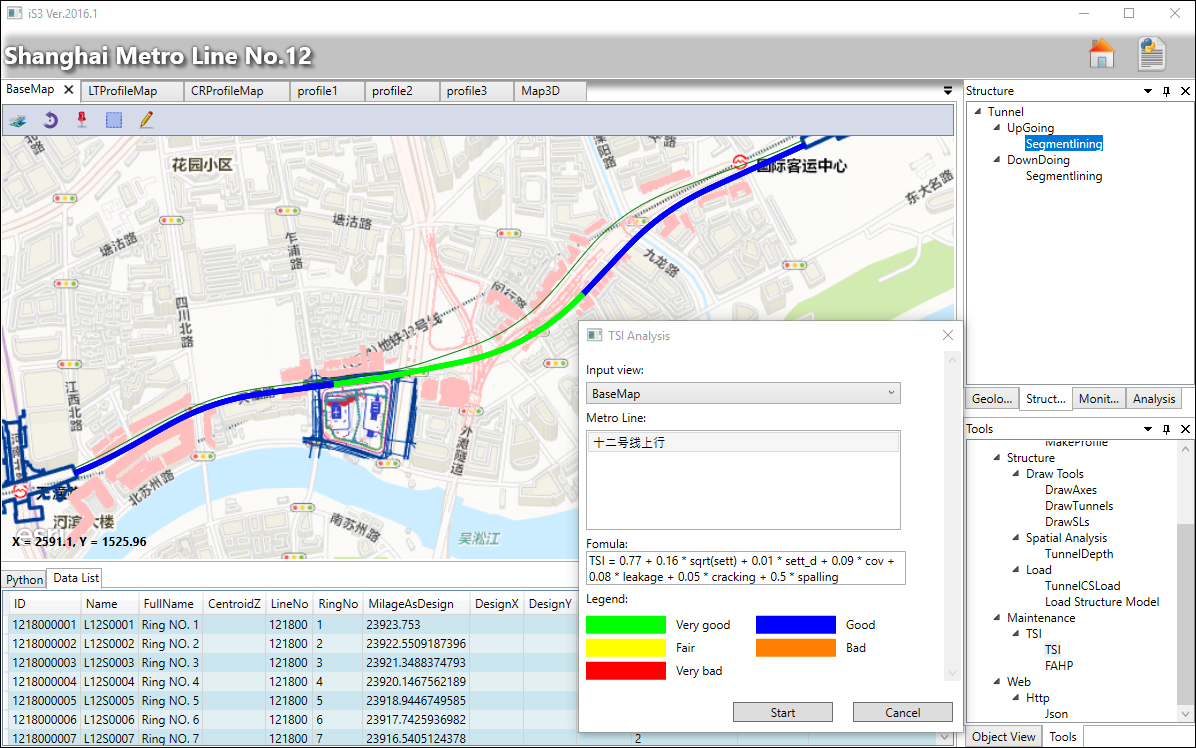
\includegraphics[width=0.9\textwidth]{chap5/desktop-tsi.png}
    \caption{盾构隧道服役性能分析}
    \label{fig:盾构隧道服役性能分析}
\end{figure}

\subsection{iS3网页端}

对于iS3-Web应用,除了采用上述的盾构隧道相关微服务分析功能以外,其GIS模型也将以服务的形式提供。首先盾构隧道工程相关的所有数据均存储在PostGIS(OSGeo,\citeyear{postgis2018})数据库中,PostGIS是一款地理数据库,具备普通关系型数据库的功能,且可存储带有坐标系的二维图形信息,采用GeoServer(OSGeo,\citeyear{geoserver2018})服务器读取数据库中的信息,并提供二维数据服务,如图~\ref{fig:GeoServer服务器}~所示。

\begin{figure}[htb!]
    \centering
    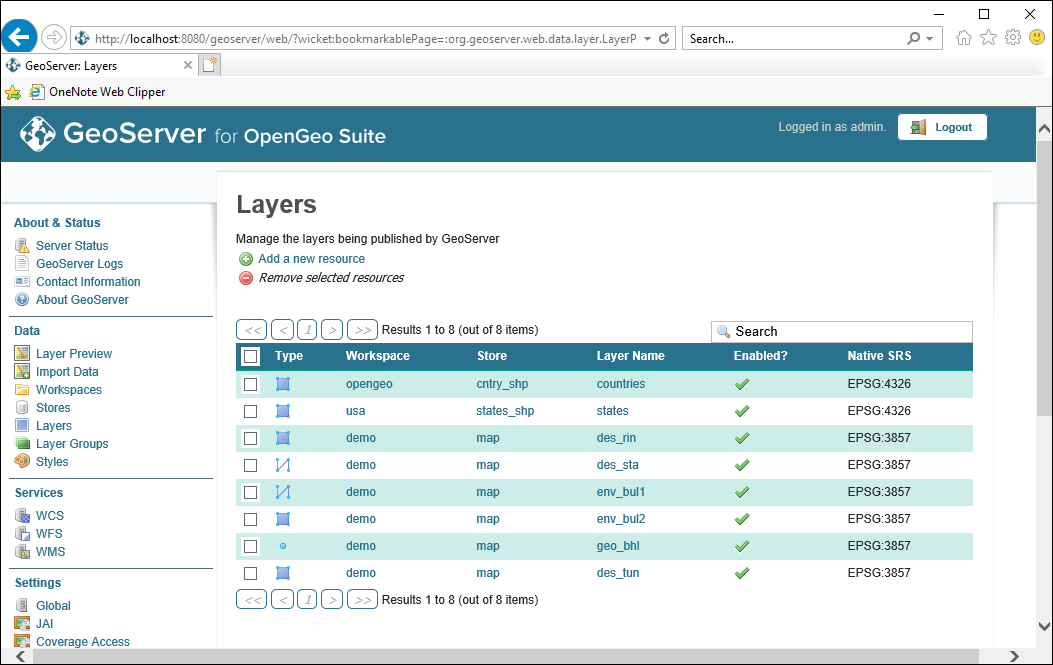
\includegraphics[width=0.9\textwidth]{chap5/geoserver.png}
    \caption{GeoServer服务器}
    \label{fig:GeoServer服务器}
\end{figure}

网页端语言自身支持HTTP请求方式,通过浏览器即可向微服务发送盾构隧道服役性能计算的请求,如图~\ref{fig:iS3Web请求服役性能分析微服务}~。目前iS3 Web仅支持数据服务查询和过滤等基础功能,如图~\ref{fig:iS3Web数据请求与编辑功能}~,采用数据库的形式存储属性信息和几何信息更便于数据的修改,修改的几何图形则由GeoServer及时渲染实时更新。同桌面端一样,网页端也可调用不同的微服务完成各种复杂分析功能,并在界面中可视化结果。

\begin{figure}[htb!]
    \centering
    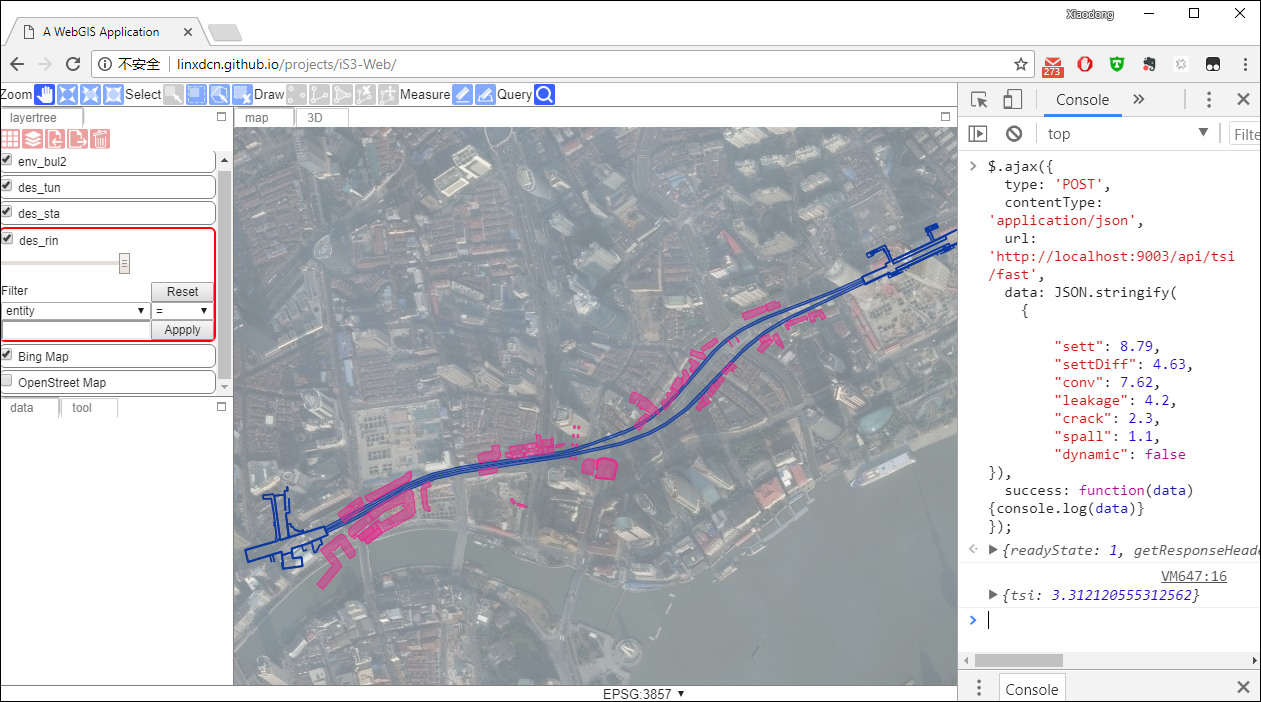
\includegraphics[width=0.9\textwidth]{chap5/iS3-Web.png}
    \caption{iS3 Web请求服役性能分析微服务}
    \label{fig:iS3Web请求服役性能分析微服务}
\end{figure}

\begin{figure}[htb!]
    \centering
    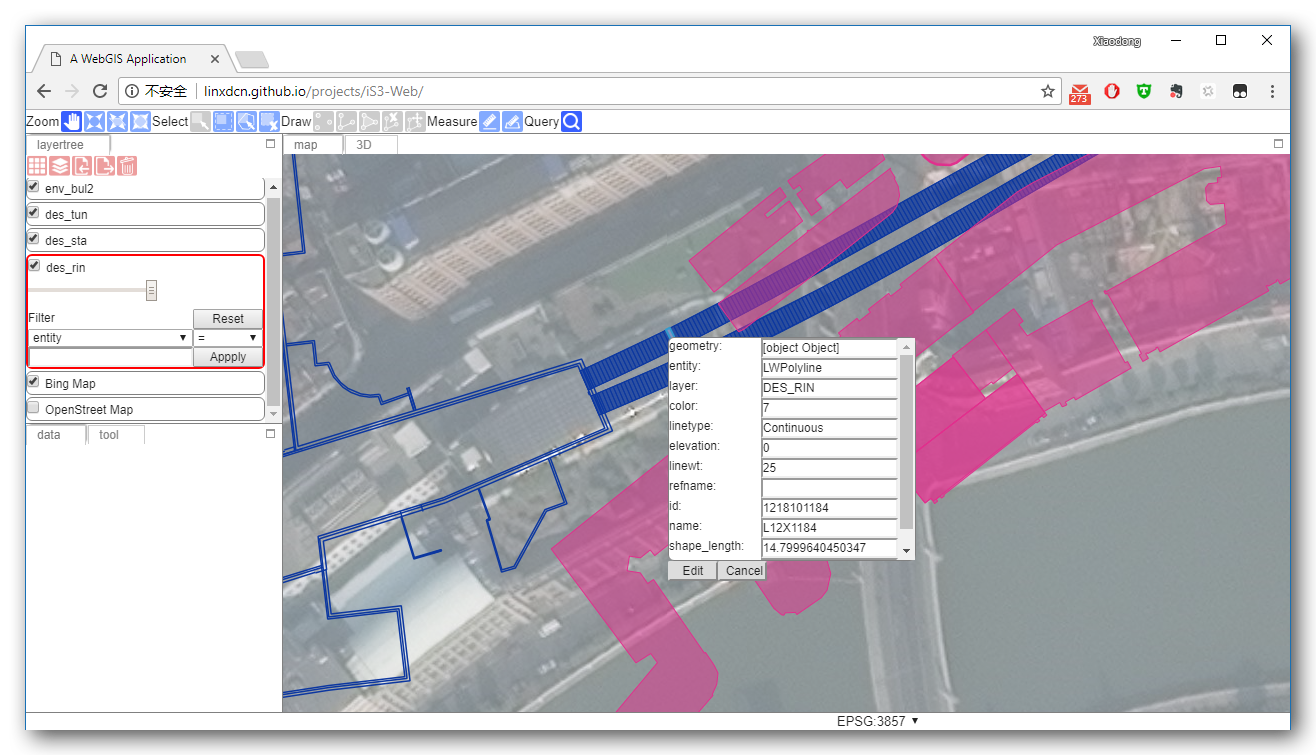
\includegraphics[width=0.9\textwidth]{chap5/iS3Web-query.png}
    \caption{iS3 Web数据请求与编辑功能}
    \label{fig:iS3Web数据请求与编辑功能}
\end{figure}

由上述的iS3 Desktop和iS3 Web两个客户端的应用可知,第~\ref{chap:service}~章的微服务架构能很好的为不同应用提供服务能力,应用层的开发主要关注请求数据的准备和响应数据的解析可视化,调用统一的微服务在分析功能更新升级时更加便捷。另外,微服务由于采用服务发现的机制,信息分析功能可快速的从不同的机器接入微服务系统,分析功能具备良好的扩展性。

%%%%%%%%%%%%%%%%%%%%%%%%%%%%%%%%%%%%%%%%%%%%%%%%%%%%%%%%%%%%%%%%%%%
\section{本章小结}

本章以上海轨道交通12号线天潼路-国际客运中心站区间为工程案例,以盾构隧道服役性能微服务为架构,描述了本文内容在工程中的应用,包括:

(1)对工程案例进行简单描述,并介绍工程的基础平台:基础设施智慧服务系统(iS3),其是全寿命数据采集、处理、表达、分析的一体化决策服务系统,包含了基础层、数据层、服务层、应用层和用户层,本文主要工作在于服务层和应用层。

(2)实现了盾构隧道服役性能评估相关的微服务,有服务发现中心和各微服务的API网关,列举浏览器、命令行和第三方客户端等的微服务请求方式,最后展示了数据服务、TSI服务和有限元服务的请求结果。

(3)在微服务基础上,开发iS3桌面端和网页端应用,介绍应用借助服务中心实现的对于盾构隧道地质勘察、结构设计、运营监测和养护维护各全寿命阶段的管理。